\clearpage
\section{Home and your role-based path}
\label{sec:correspondence-feature-home}

Home brings together work and follow-up destinations. Start with your assigned responsibility: preparing a letter, reviewing a draft, approving, receiving, or registry work. These are workflow responsibilities, not role names that must be created verbatim.

\begin{rcnote}[Example: Horizon]
Omar checks his capacity at ① and opens the tray through ② to continue his visit-request draft. Sarah uses “Awaiting my approval” at ③ when a request reaches her; her position alone does not make her the approver of every letter.
\end{rcnote}
\begin{figure}[H]
\centering
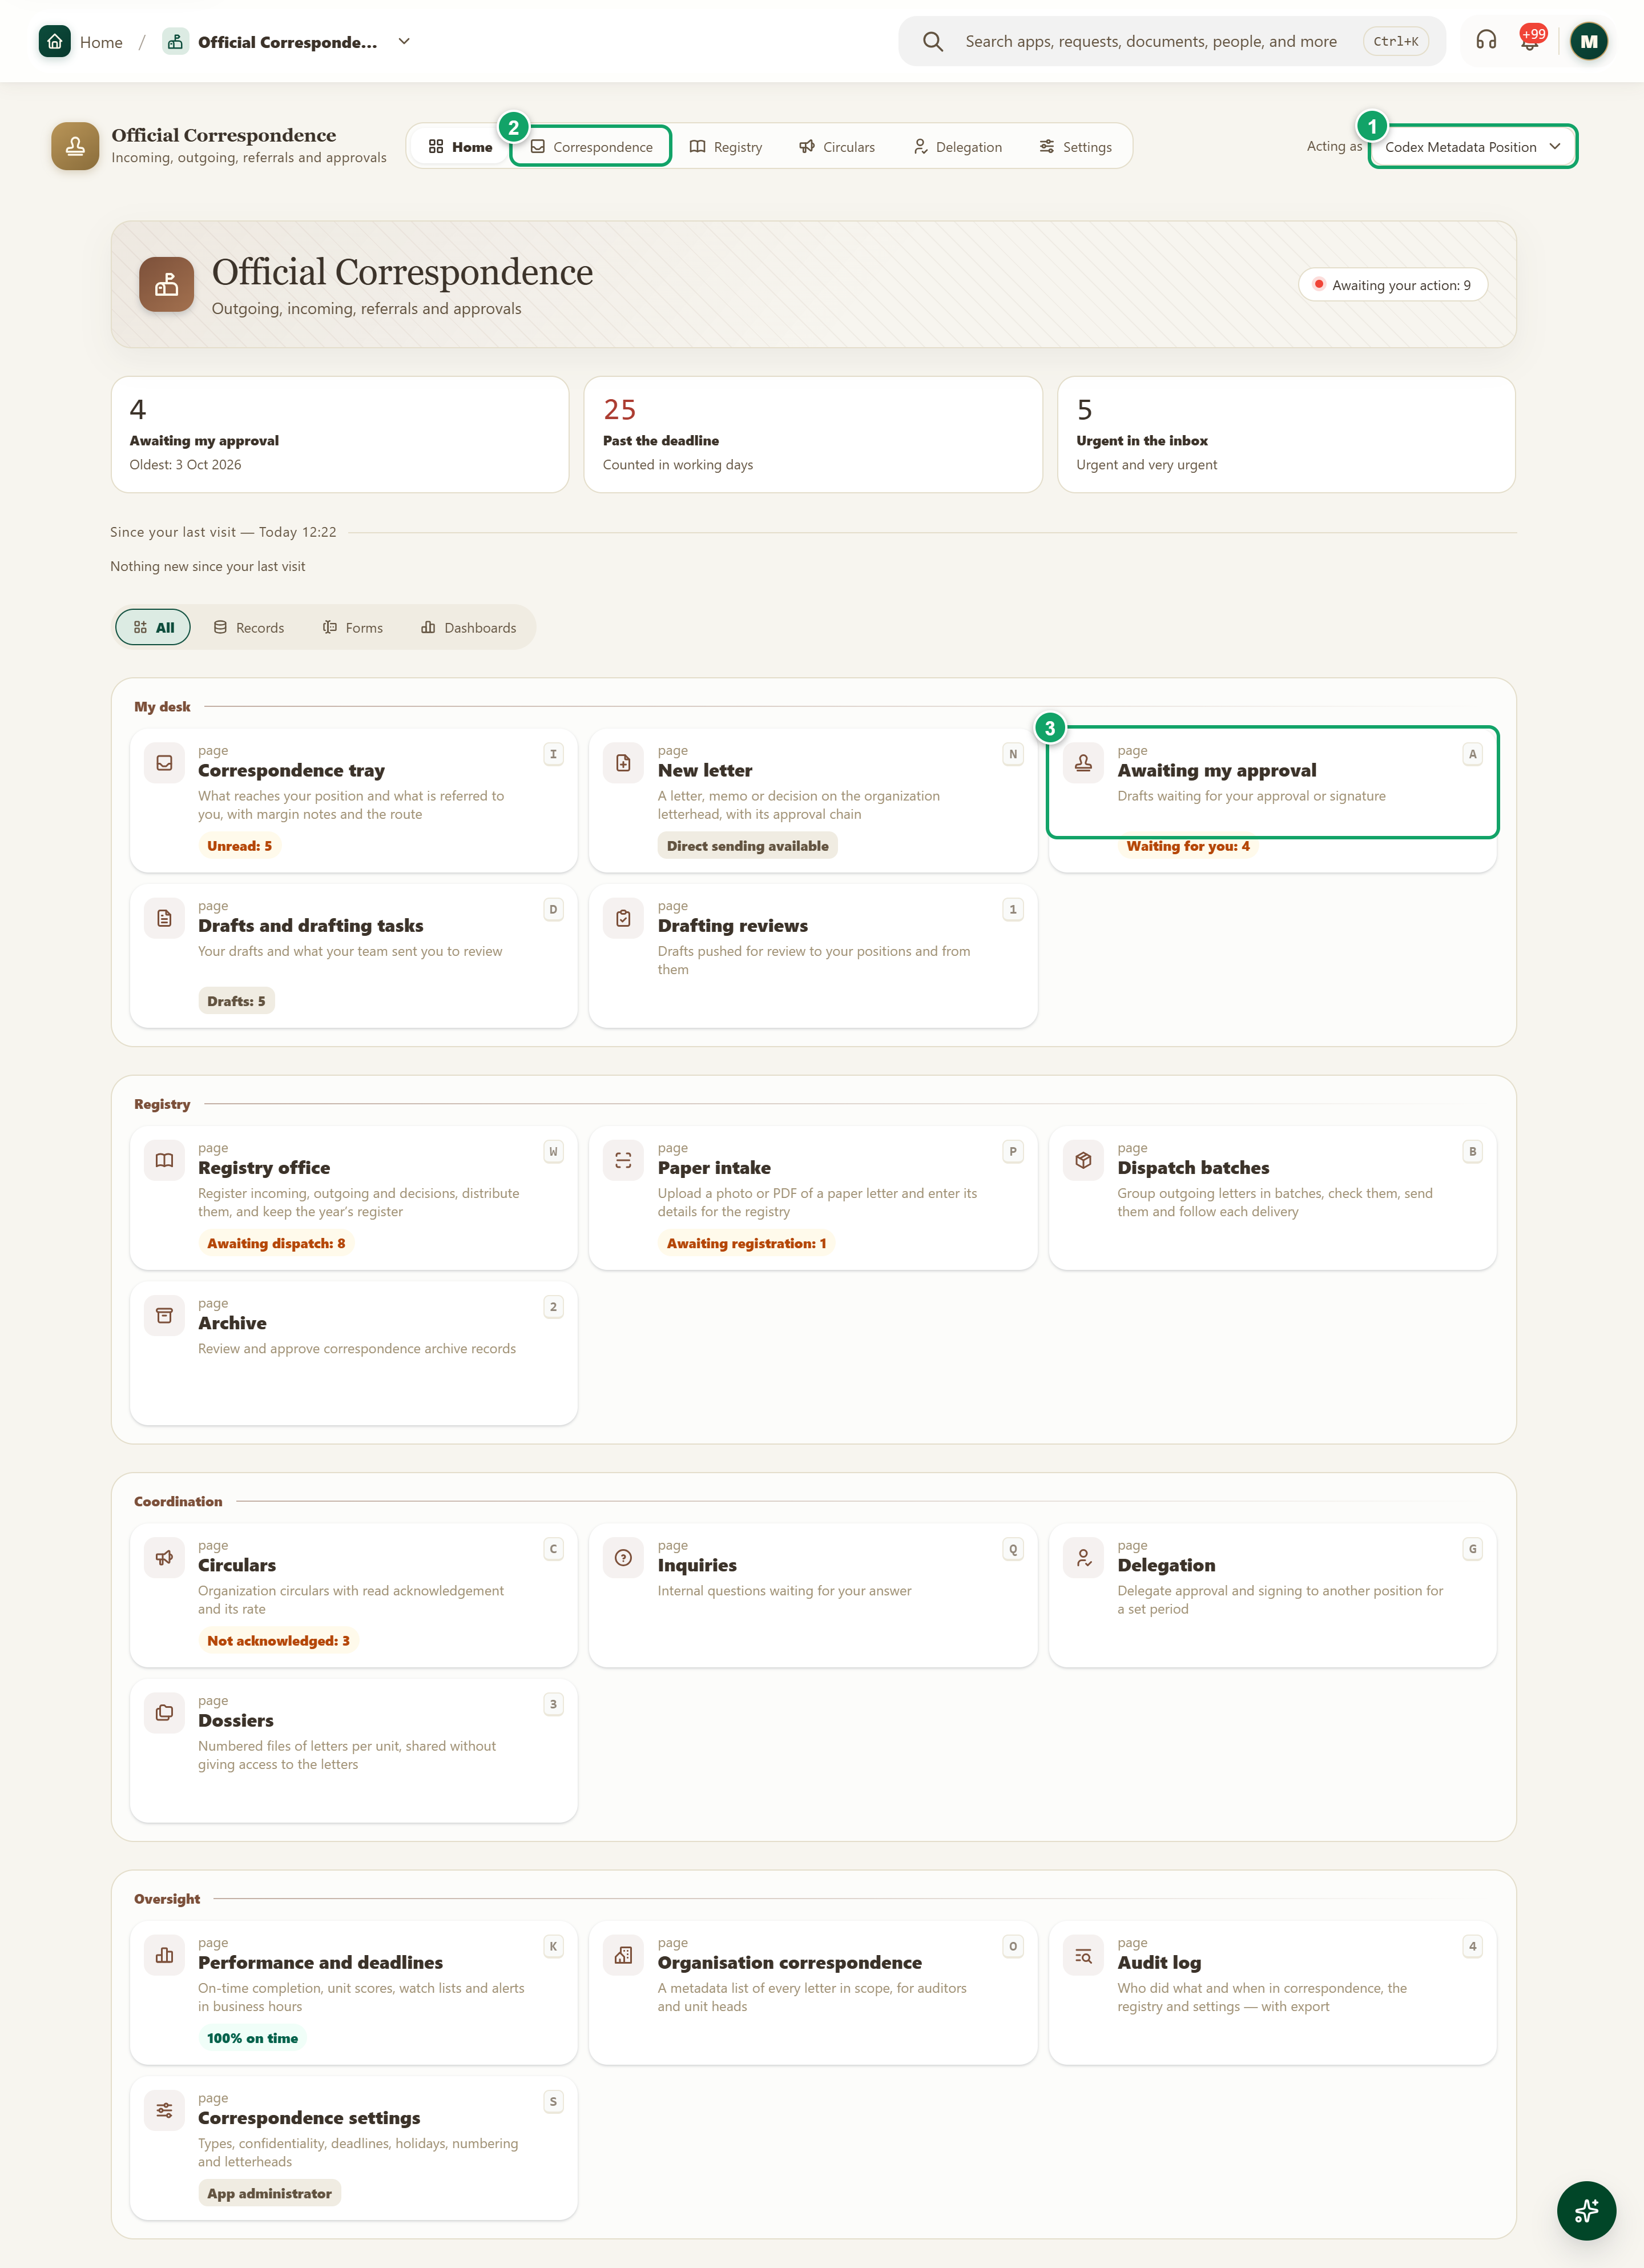
\includegraphics[width=0.95\linewidth,height=0.72\textheight,keepaspectratio]{figures/screens/ch07-home-en.png}
\caption{Home and work destinations}
\label{fig:correspondence-home-screen}
\shotnote{Home groups work destinations by responsibility and provides counts to guide follow-up. These are test records, not the Horizon example. ① “Acting as”: selects the position you act as. ② “Correspondence”. ③ “Awaiting my approval”.}
\end{figure}


\begin{table}[H]
\centering
\caption{Where should you start?}
\label{tab:correspondence-responsibilities}
\begin{tabularx}{\linewidth}{R{4.2cm} Y}
\rcHeaderRow
\thh{Responsibility} & \thh{Starting point}\\
Preparer & Use “New letter” to start and “Drafts and drafting tasks” to continue saved work.\\
Draft reviewer & Open “Drafting reviews” for drafts pushed for review. Draft review is distinct from final approval.\\
Approver & Open “Awaiting my approval” and inspect the request addressed to you.\\
Recipient & Open “Correspondence tray”, then “Inbox”; use “Copies for information” to distinguish information copies.\\
Registry clerk & Start at “Registry office” when you have registration permission.\\
Administrator & Open “Correspondence settings” when you have administration permission.\\
\end{tabularx}
\end{table}

\begin{enumerate}
\item Open “Official Correspondence” from the app launcher.
\item Read “Acting as”, then open the destination for your responsibility in the table.
\item Check the page title and folder: “Awaiting my approval” and “Drafts and drafting tasks” lead to views within the tray.
\end{enumerate}

\textbf{Check:} Name your responsibility and starting point before continuing. If Registry or Settings is absent, check your permission with the administrator; a missing destination does not by itself mean the app is broken.

\clearpage
\section{Capacity and permissions}
\label{sec:correspondence-feature-capacity}

Your capacity is the position in whose name you handle correspondence. Your account may have several positions, and a valid delegation may make another position available. Switching capacity does not grant new permission; available actions still depend on the letter, assignment, delegation and permissions.

\begin{rcnote}[Example: Horizon]
Omar selects his “Operations Coordinator” position at ①, then opens “Drafts” at ② to follow his visit request. If later delegated another position, he distinguishes work on its behalf from work in his own position.
\end{rcnote}
\begin{figure}[H]
\centering
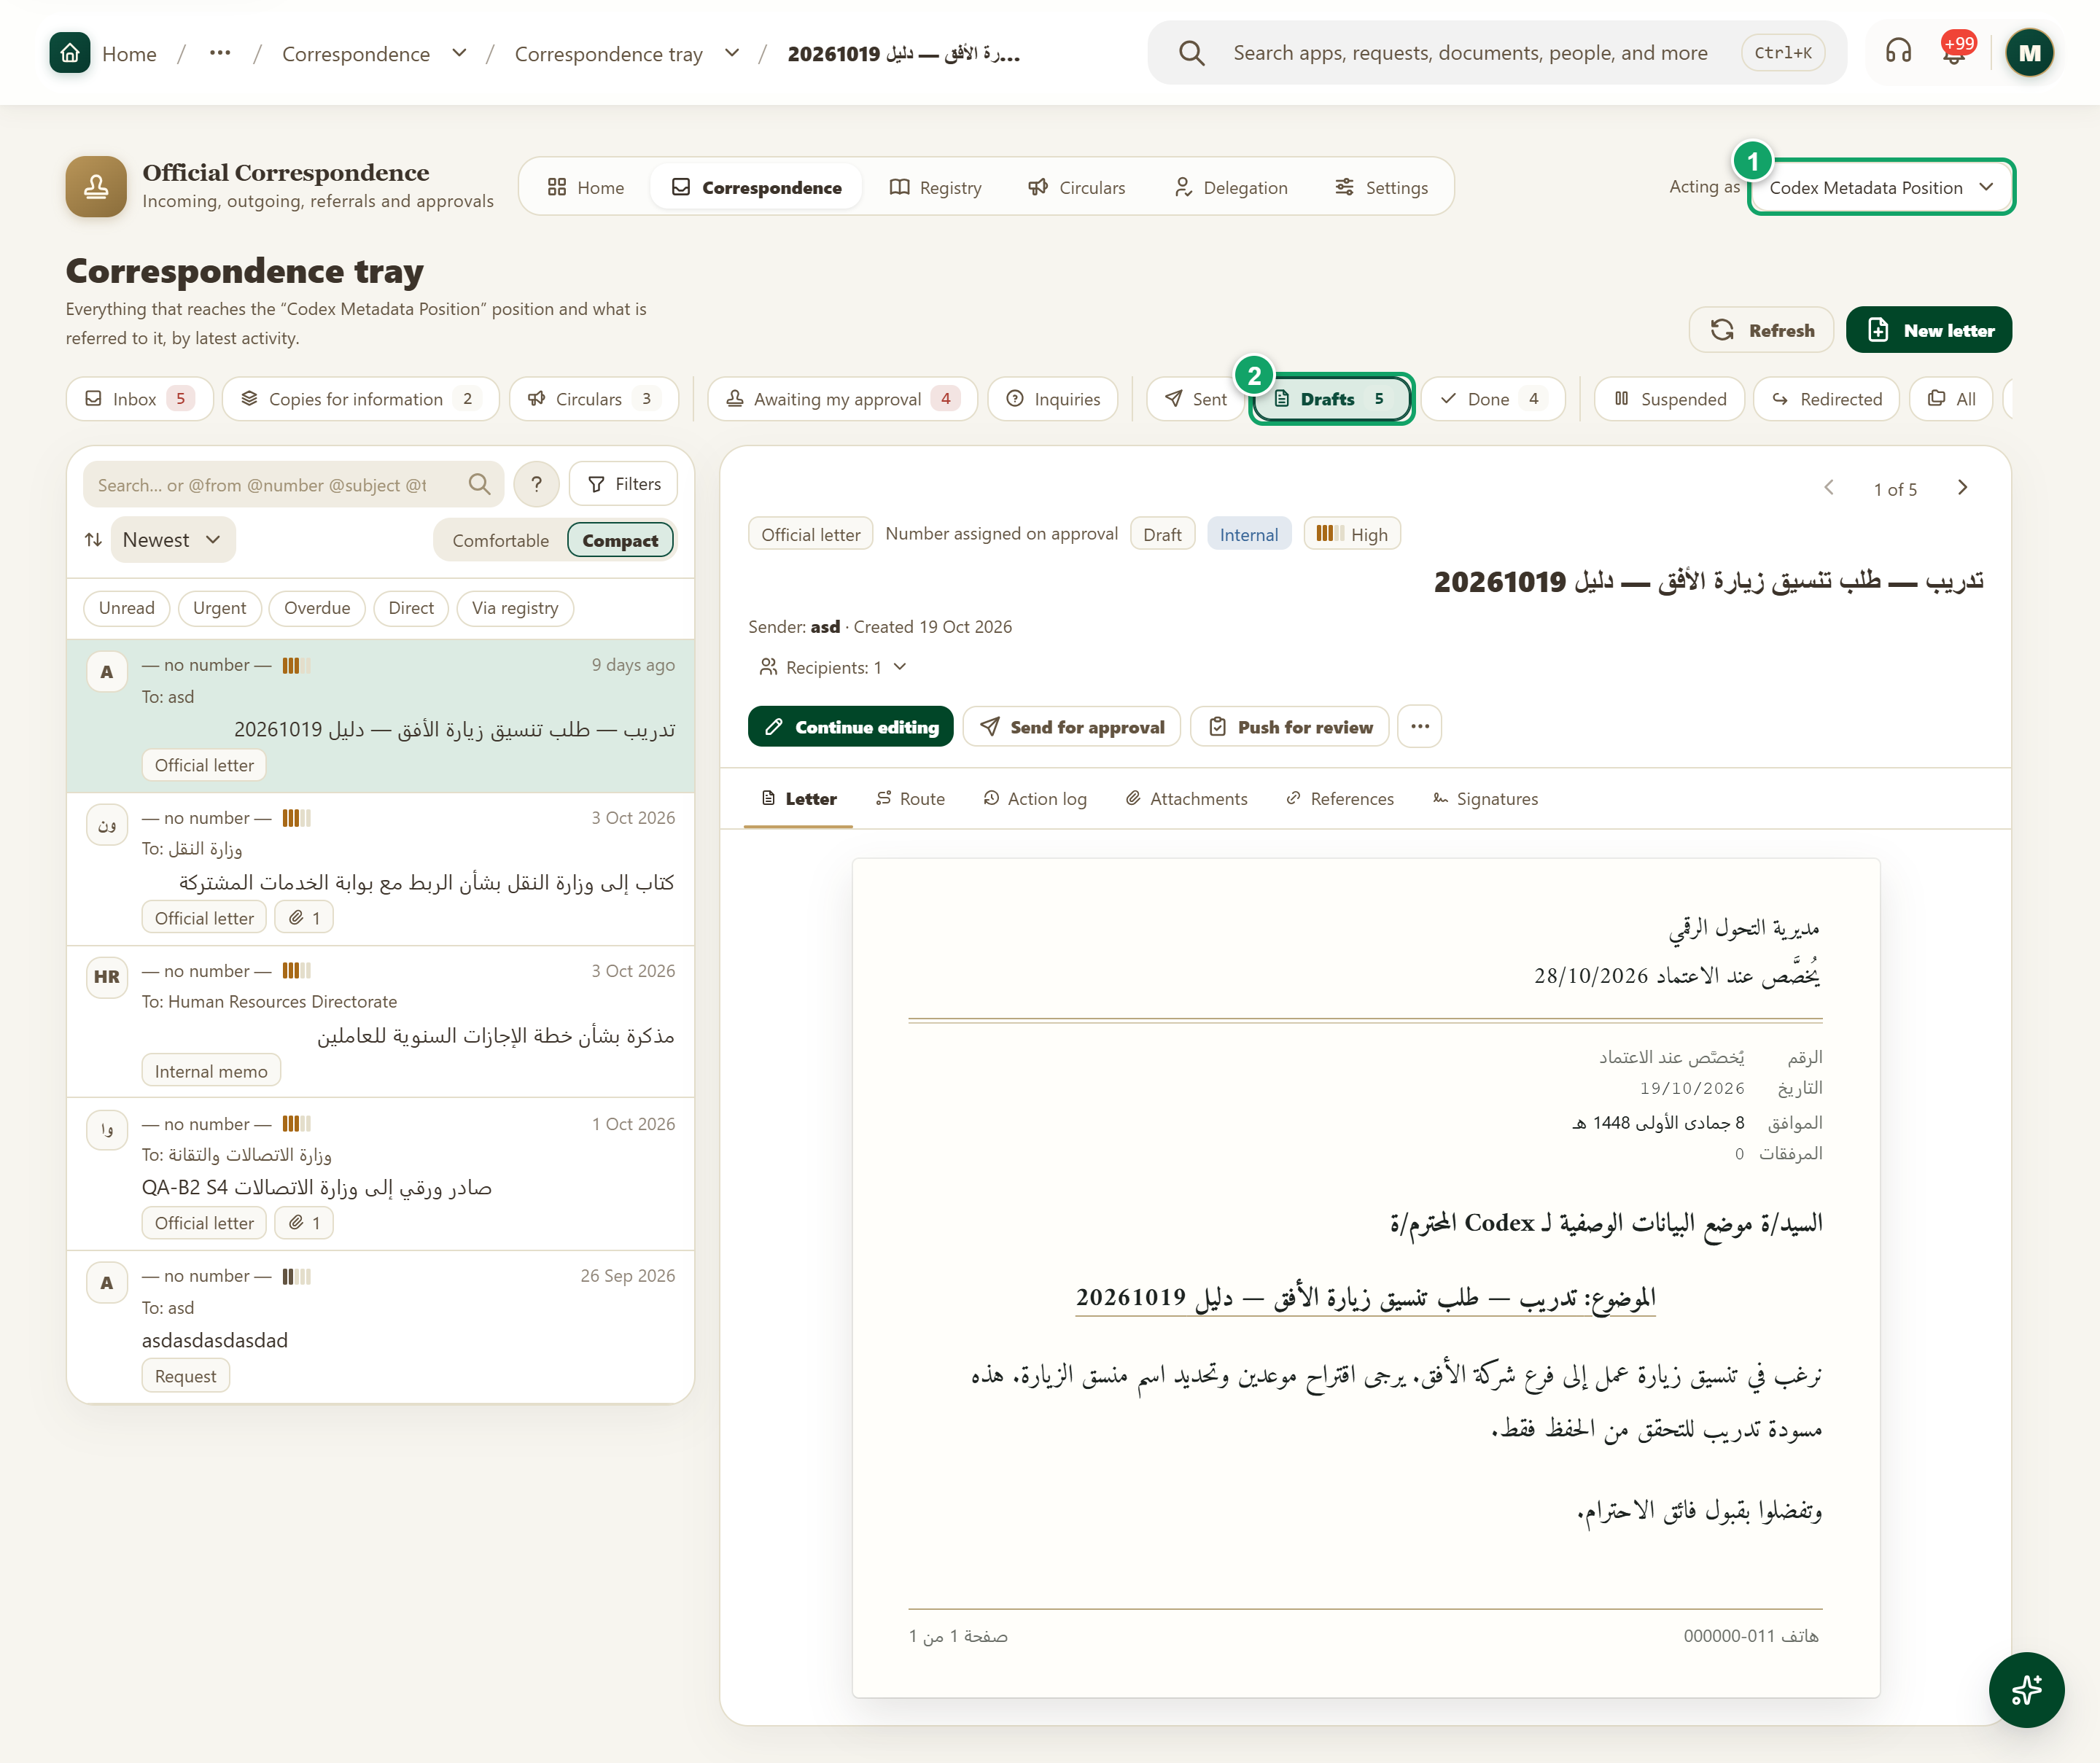
\includegraphics[width=0.95\linewidth,height=0.72\textheight,keepaspectratio]{figures/screens/ch07-capacity-en.png}
\caption{Capacity and the Drafts folder}
\label{fig:correspondence-capacity-screen}
\shotnote{The image shows the selected position and folder context with a test draft open. A draft in the tray has not necessarily been submitted for approval. ① “Acting as”: selects the position before following its work. ② “Drafts”.}
\end{figure}


\begin{enumerate}
\item Open “Official Correspondence” and locate “Acting as”.
\item If a position selector appears, choose the required position and read its selected name. With one available position, its name appears without a switcher.
\item When delegated, check “On behalf of” and the delegation expiry date.
\item Open “Correspondence tray” and check the position context before choosing a letter.
\end{enumerate}

\textbf{Check and recover:} State which position you are acting as and whether it is delegated. If the required position is absent, ask for your assignment or delegation validity and conditions to be checked; do not work under a different position to bypass the problem.

\clearpage
\section{The tray and the letter lifecycle}
\label{sec:correspondence-feature-tray}

The “Correspondence tray” groups available work into folders. A folder helps you find work, while a status describes the letter’s stage. “Awaiting my approval” is a personal work view, and issuance does not by itself prove delivery or completion.

\begin{rcnote}[Example: Horizon]
Sarah opens “Inbox” at ① to find a letter about the Aleppo branch visit, then searches for its subject at ②. She uses “Filters” at ③ if she needs to narrow the results and reloads with ④ before checking the result.
\end{rcnote}
\begin{figure}[H]
\centering
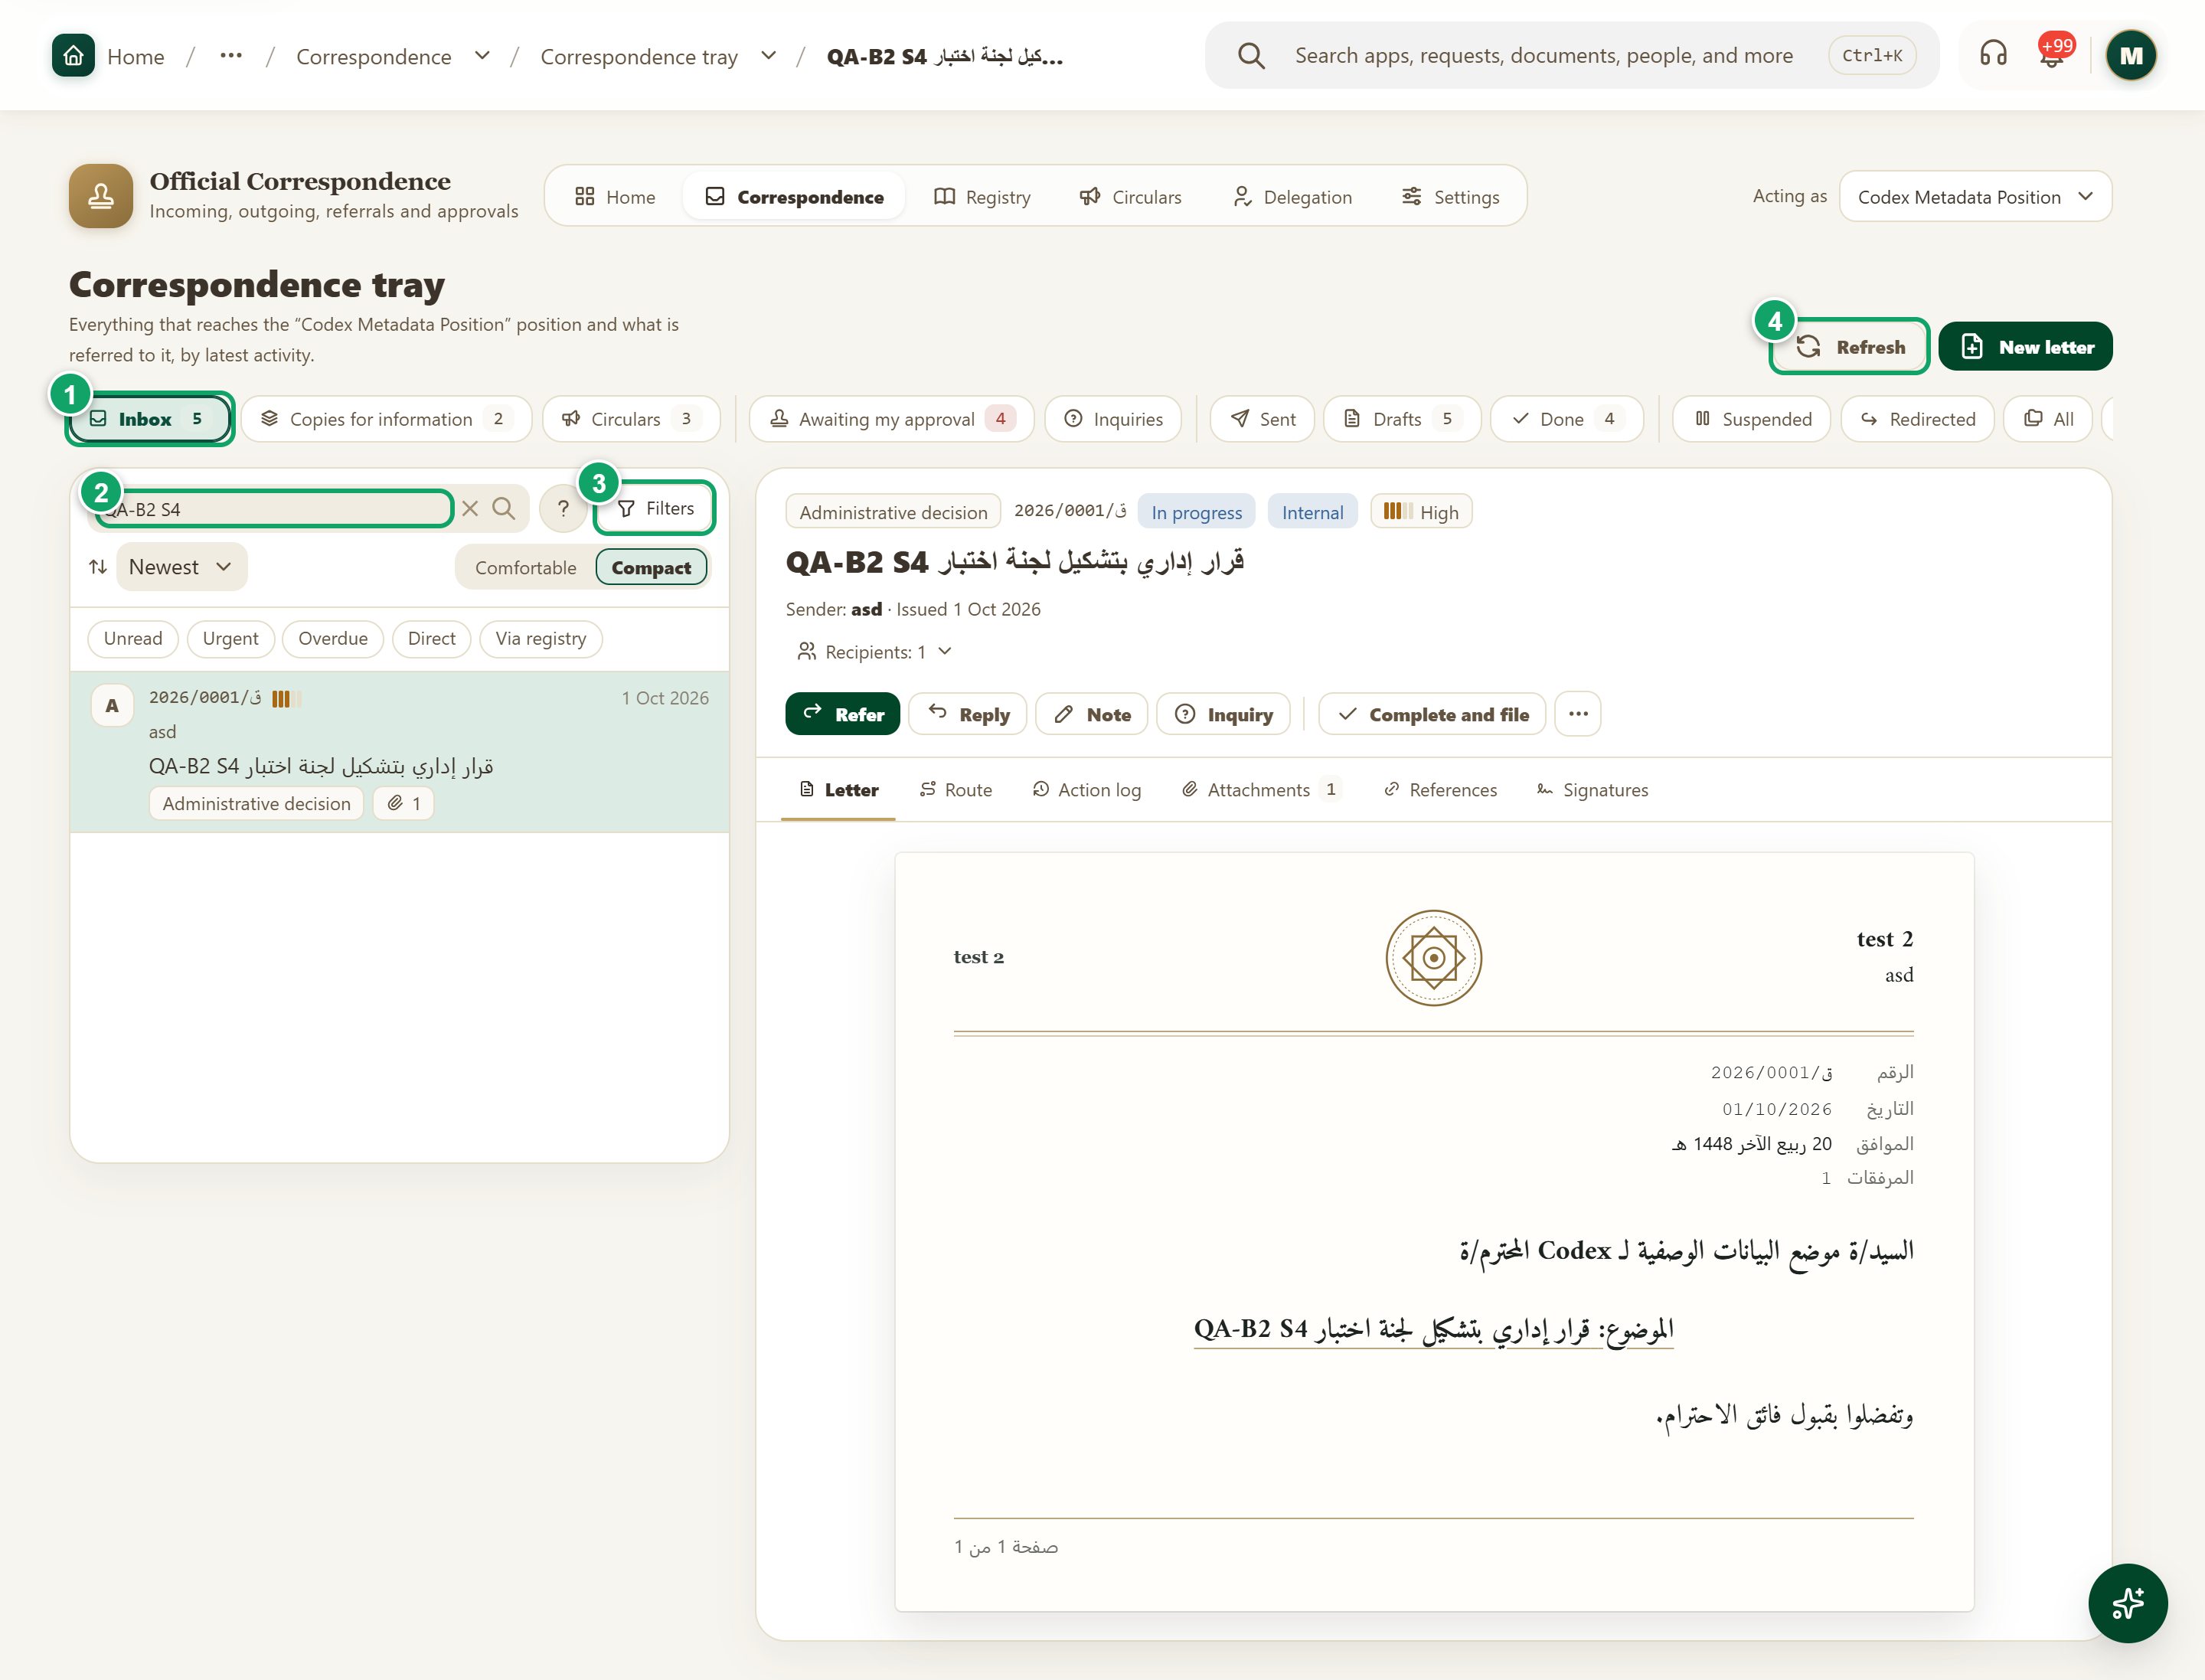
\includegraphics[width=0.95\linewidth,height=0.72\textheight,keepaspectratio]{figures/screens/ch07-tray-en.png}
\caption{Searching the correspondence tray}
\label{fig:correspondence-tray-screen}
\shotnote{The image shows a specific search result and an open test letter, allowing you to distinguish status, priority and confidentiality. Searching narrows the list without changing the letter’s status. ① “Inbox”. ② The search field finds a known subject. ③ “Filters”. ④ “Refresh”.}
\end{figure}


\begin{table}[H]
\centering
\caption{How to read a letter’s information}
\label{tab:correspondence-reading}
\begin{tabularx}{\linewidth}{R{4.2cm} Y}
\rcHeaderRow
\thh{Information} & \thh{What does it tell you?}\\
Letter type & Classifies the letter using types configured by the organization; available types can differ between organizations.\\
Status & Labels include “Draft”, “Awaiting approval”, “Returned for changes”, “Issued”, “In progress”, “Completed”, “Rejected” and “Void”. They are not one mandatory sequence.\\
Priority & Labels such as “Urgent” and “Very urgent” help prioritize follow-up; they do not grant extra permission.\\
Confidentiality & Identifies access classification, such as “Public”, “Internal” or “Secret”. It is distinct from priority.\\
Deadline & Helps identify work needing attention; check the due date and whether the deadline is paused.\\
\end{tabularx}
\end{table}

\begin{enumerate}
\item Open “Correspondence tray”, then select “Inbox”, “Drafts” or “Awaiting my approval” for your work.
\item Search for a word from a known letter’s subject and inspect the results. You can use “Filters” or quick filters such as “Unread” and “Urgent”.
\item Clear the search and filter if the letter is missing, then check the capacity and folder. Use “Refresh” to reload the list.
\item Open an available letter and read its subject, status, priority and confidentiality before taking action.
\end{enumerate}

\textbf{Practice and check:} Switch from “Inbox” to “Drafts” and back, then search and clear the search. Confirm the folder changes and the list returns. If it is empty, record that observation rather than concluding the organization has no letters. If “The folder could not be loaded” appears, use “Try again”; a loading error is not an empty search result.
